\chapter{Design and Implementation}
\label{chp:design_and_implementation}

The hardware design of the transiently-powered robot is presented in Section \ref{sec:dai_hardware_design}.
In Section \ref{sec:dai_control_design} the controller will be explained that allows the robot to perform controlled movements without external feedback.
Finally, Section \ref{sec:dai_software_implementation} introduces the software implementation that enables the robot to execute a movement despite regular power interrupts. 

\section{Hardware Design}
\label{sec:dai_hardware_design}
The first step in the hardware design is to evaluate what components are required for the robot to have basic navigation capabilities. 
Commercially available low power components have been evaluated, where the main criteria was a low minimal supply voltage of 2.0\,V to function with a system voltage of 2.2\,V.
This section will explain each part of the robot in more detail.
A complete overview of the robot is shown in Figure \ref{fig:robot_overview} and a complete assembled robot with WISP and solar panel is shown in Figure \ref{fig:robot_picture}.

\vspace{1em}
\begin{figure}[h!]
	\centering
	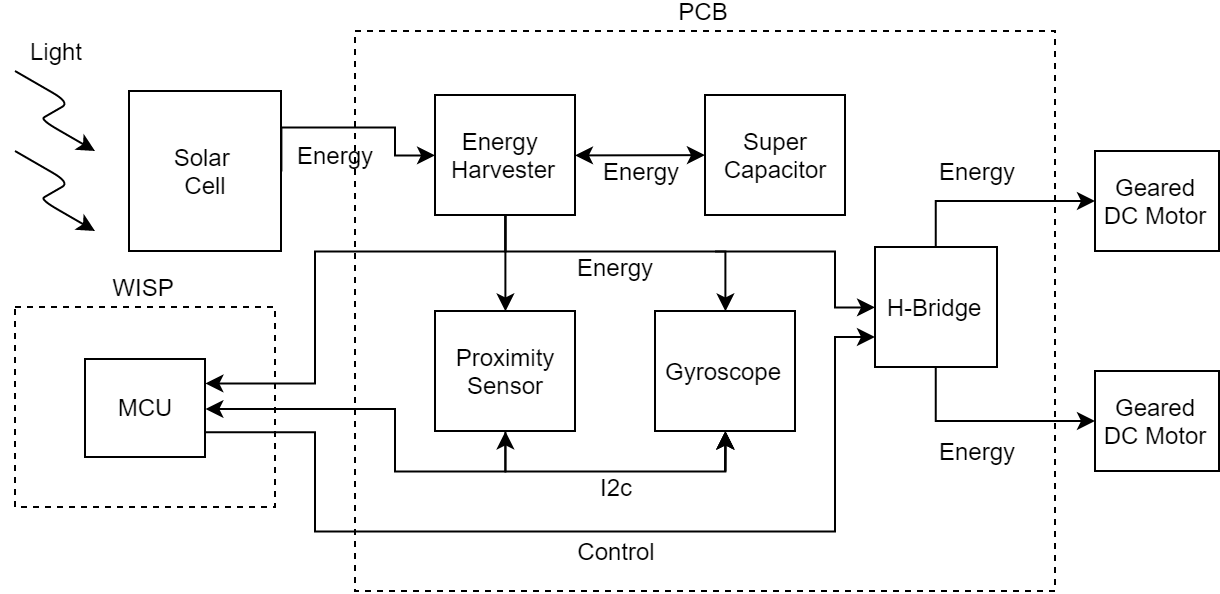
\includegraphics[width=0.9\textwidth]{pics/schematic_robot_v2.png}
	\caption{Schematic overview of the transiently-powered robot.}
	\label{fig:robot_overview}
\end{figure}

\begin{figure}[h!]
	\centering
	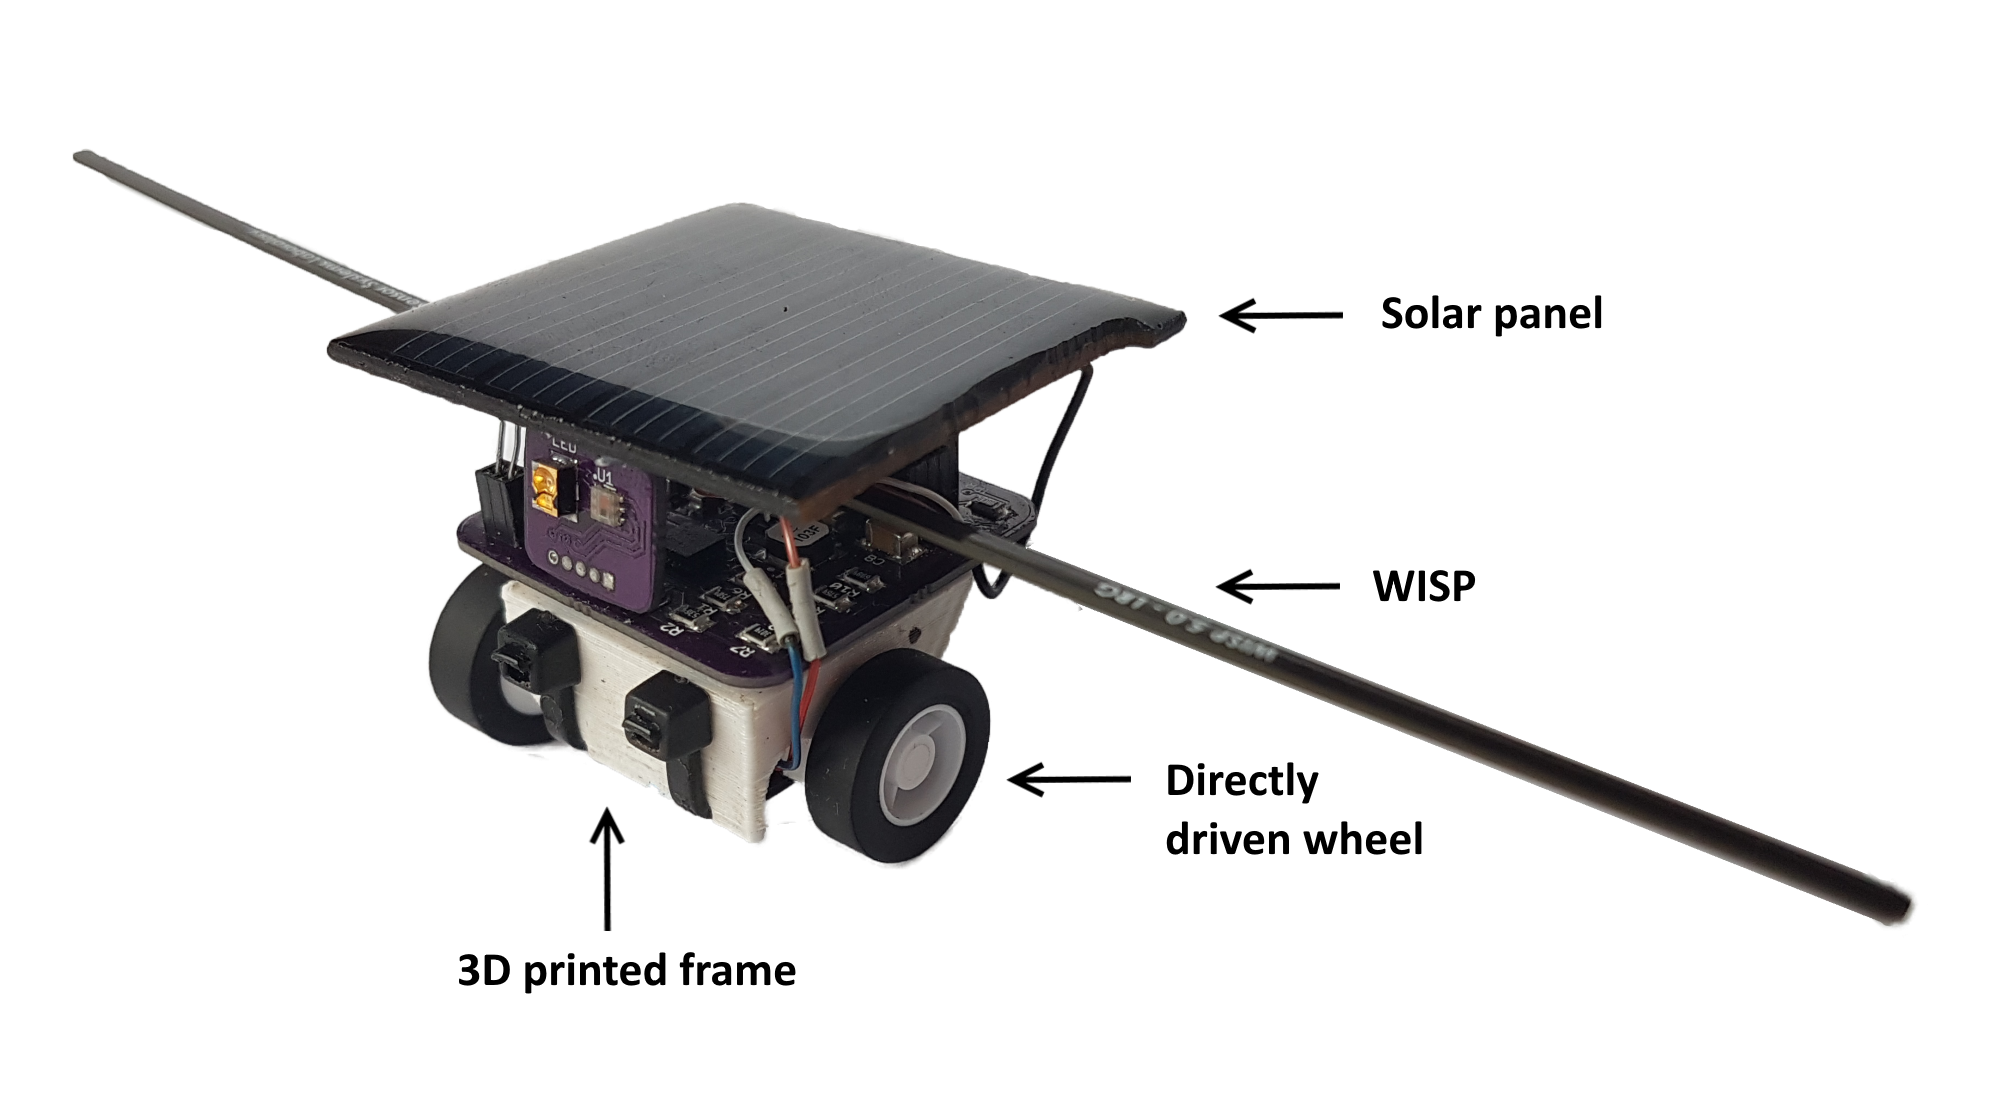
\includegraphics[width=0.9\textwidth]{pics/tp_robot2.png}
	\caption{The complete robot with WISP and solar panel.}
	\label{fig:robot_picture}
\end{figure}

\subsection{Energy Harvesting and Storage}
Energy is harvested from light using two IXYS SLMD121H04L-ND solar cells~\cite{ixolar_slmd121h04l_2017} in parallel, as determined in Section \ref{sec:pre_energy_source_selection}.
The solar cells will be connected to a Texas Instruments BQ25570 energy harvester~\cite{bq25570_2017} which stores the harvested energy in a 22\,mF - 4.5\,V supercapactor from AVX~\cite{avx_bestcap_2017}.

\subsection{Computation}
\label{sec:dai_computation}

The robot is designed around a WISP 5 \cite{wisp5_wiki_2017}, a battery-free platform for low power sensing, computation and communication.
This platform has the ability to communicate with RFID readers and is powered by the carrier signal emitted by the reader.
However, the communication range and the power that can be harvested is limited. 
Only the MCU from the WISP is currently being utilized: a Texas Instruments MSP430FR5969 ultra low power microcontroller.
This MCU can operate at 16\,MHz and features 64\,KB FRAM, 2\,KB SRAM and 40 IO-ports \cite{msp430fr5969_2017}.

%Therefore communication is currently not implemented and a different energy source for harvesting will be used as described in Section \ref{sec:pre_energy_harvesting_storage}.

\subsection{Sensing}
\label{sec:dai_sensing}

The robot has access to basic sensors which can be interfaced trough I2C.
For detecting obstacles in front of the robot, a Maxim Integrated MAX44000 proximity sensor~\cite{max44000_2017} was added of the robot facing forward.
The sensor switches an IR led at high frequency to reduce the power consumption.
Because the sensor is based around a photo-diode it can be used to measure the amount of ambient light as well.
To allow for local motion feedback, the robot has a Bosch Sensortec BMG250~\cite{bosch_bmg250_2017} low power triaxial gyroscope to measure yaw-rate.

\subsection{Locomotion}

Sub-micro plastic planetary gearmotors from Precision Microdrives~\cite{gearmotor_206-110_2017} are chosen to provide locomotion to the robot, as described in Section \ref{sec:pre_locomotion_selection}.
Two motors are mounted diagonally opposite from each other in a 3D printed frame making the robot as compact as possible, and the differential drive configuration allows steering.
Small plastic wheels with rubber tires are mounted directly on each of the motor shafts.
Behind these two motors a free running caster wheel is mounted to the frame, acting as a third support point for the robot.

\subsection{Motor Control}
\label{sec:dai_motor_control}

The speed and the current consumption of each motor can be controlled individually using PWM.
The MCU can use the H-bridge to enable, disable and control the direction of rotation of each individual motor.
MCU output ports are limited in the amount of current that they can supply.
MOSFETs inside a Texas Instruments DRV8836 dual H-bridge~\cite{drv8836_2017} allow efficient regulation of larger currents to the motors.

\subsection{Integration}
Now that all the parts have been chosen, they can be connected together to form the robot.
A Printed Circuit Board (PCB) has been designed using EAGLE PCB design and schematic software.
The PCB increases stability, eases connection and reduces of the total weight of the robot.
Additionally, a PCB was required because of use of small size ICs (no lead packaging).
A detailed schematic of the PCB can be found in Appendix \ref{app:schematic_robot}.

An overview of both the top and bottom side of the PCB is shown in Figure \ref{fig:pcb_robot}.
The PCB contains headers to connect the solar panel and headers to connect all the required pins from the WISP.
An additional header is available to connect a battery for testing purposes.
All the large components are mounted externally: the solar panel, WISP and the motors.
%Most reference designs are extendable but this adds complexity, while weight and size are the main constraints in the design of this robot.

%The top of the PCB contains all the surface mount components that are soldered to the PCB using a reflow oven. 
%When the boards come out of the oven, the headers, motors and supercapacitor are soldered to the boards by hand.

\begin{figure}[h!]
	\centering
	\begin{subfigure}[b]{0.45\textwidth}
		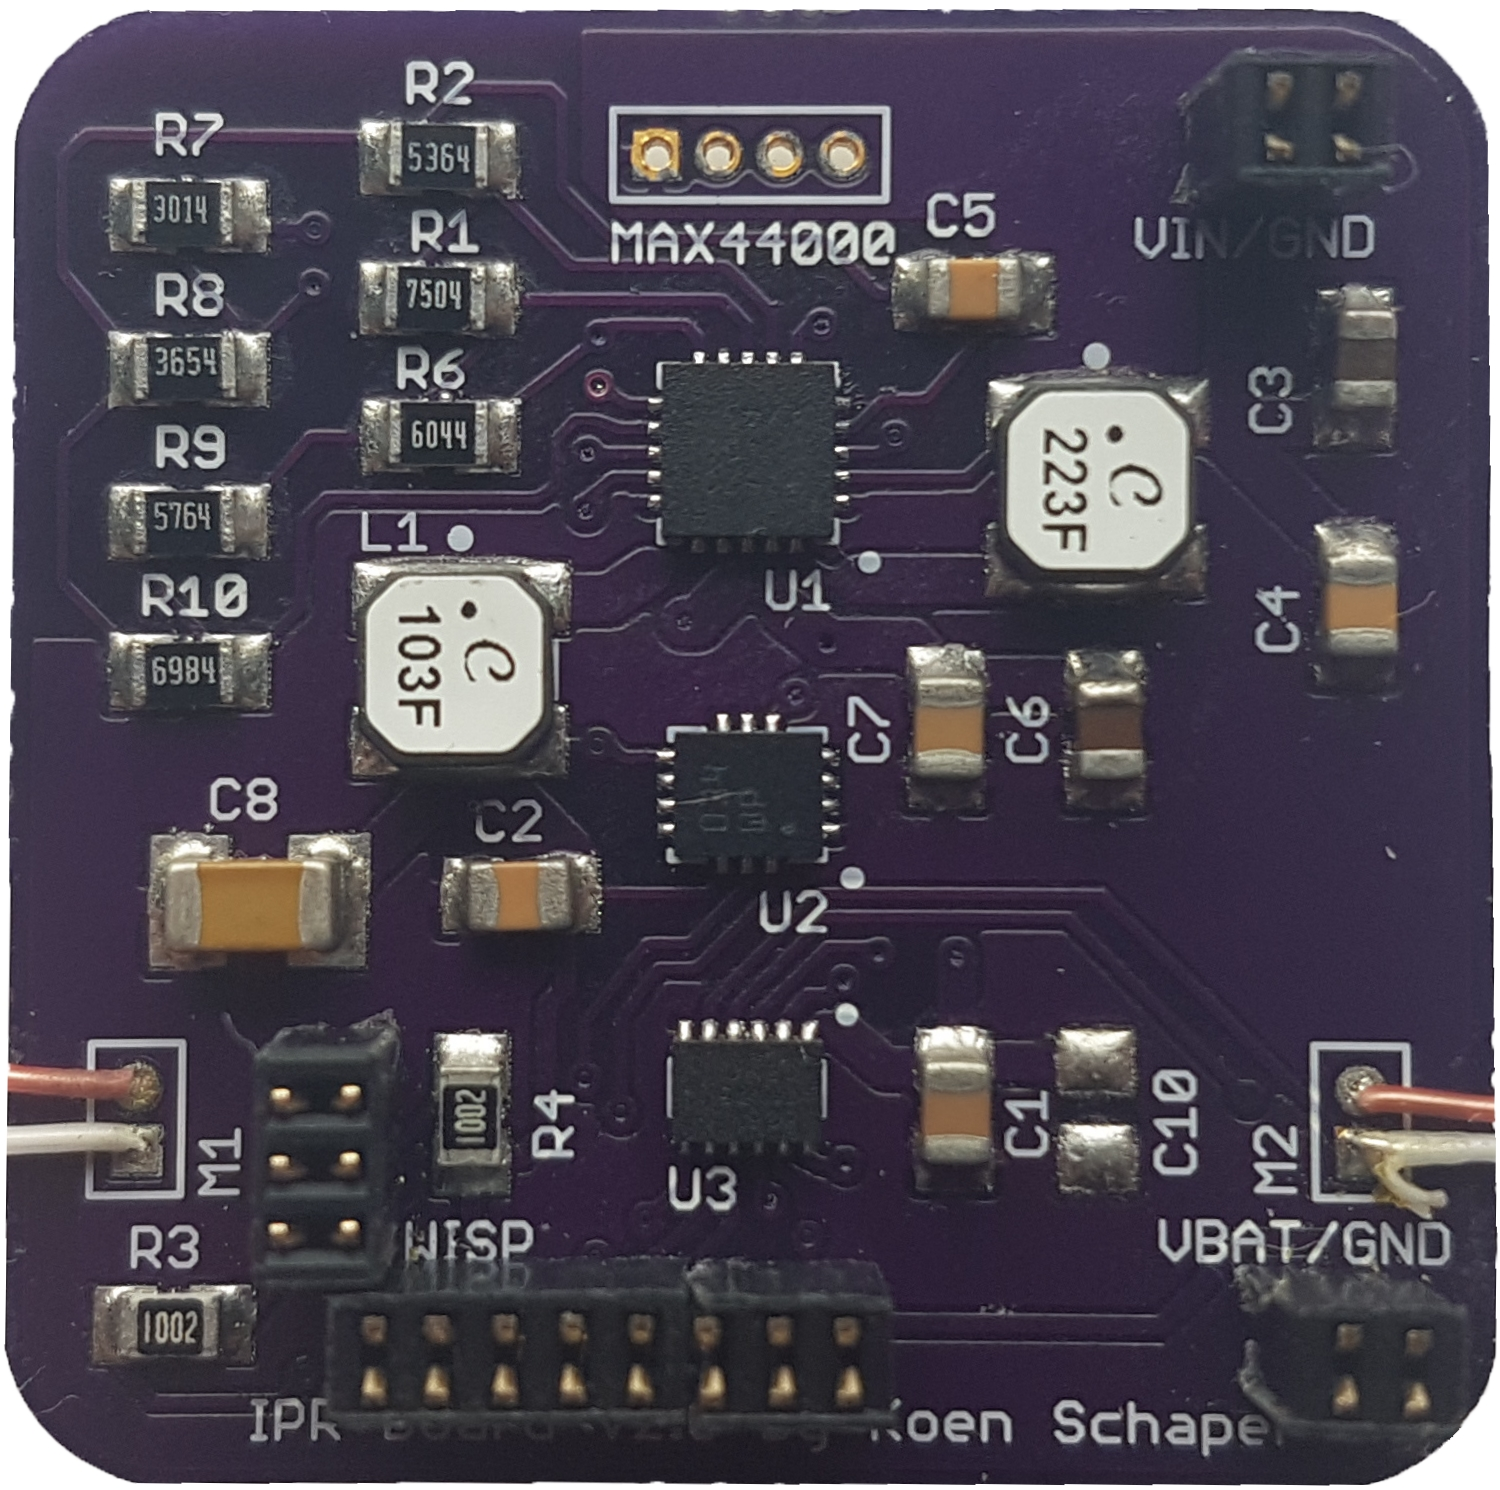
\includegraphics[width=\textwidth]{pics/pcb_front.jpg}
		\caption{Top side of the PCB}
		\label{fig:pcb_robot_front}
	\end{subfigure}
	\qquad
	\begin{subfigure}[b]{0.45\textwidth}
		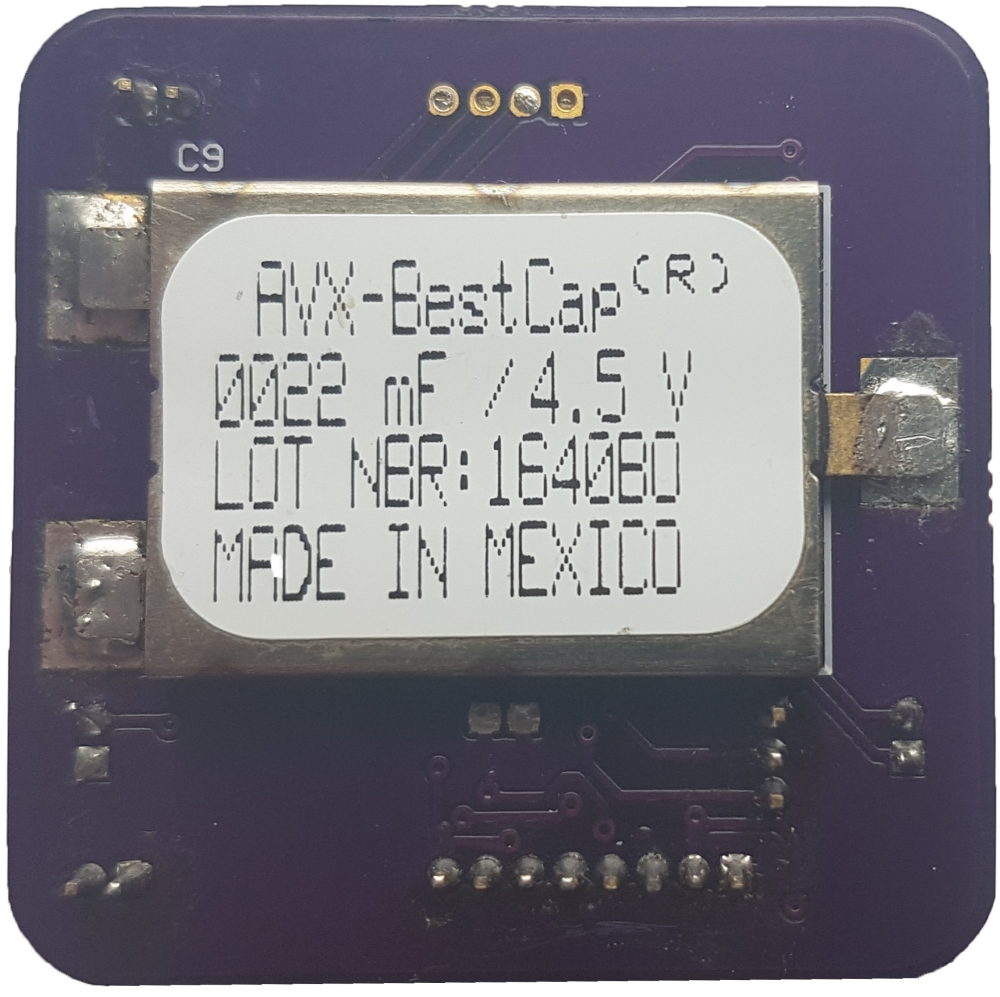
\includegraphics[width=\textwidth]{pics/pcb_back.jpg}
		\caption{Bottom side of the PCB}
		\label{fig:pcb_robot_back}
	\end{subfigure}
	\caption{The PCB designed for the robot, on the top side of the PCB the ICs are marked, harvester (U1), gyroscope (U2) and H-bridge (U3). The bottom side only contains the supercapacitor.}
	\label{fig:pcb_robot}
\end{figure}

\subsection{Energy Expenditure}

The average current consumption by each component was measured with a Monsoon Power Monitor~\cite{monsoon_powermonitor_2017}.
The measurement is performed as follows: first a two second current trace was recorded of the current consumed by the MCU on the WISP.
The MCU was then used to enable each component individually, followed by a two second current measurement with the enabled component.
The average of each current trace is calculated, and the current consumed by the microcontroller subtracted from the current consumed by each component.
The measurement result is provided in Table \ref{tab:avg_cur_comp}.

% Make a overview of the cost to build a robot

\begin{table}[t]
	\centering
	\begin{threeparttable}
		\caption{Average consumed current for each individual component on the PCB at 2.2\,V.}
		\label{tab:avg_cur_comp}
		\begin{tabular}{|l|l|} 
			\hline
			Part & Active Current \\
			\hline\hline
			Proximity sensor & 119 \textmu A \\
			Gyroscope & 848 \textmu A\\	
			Microcontroller @ 8MHz & 522 \textmu A\\
			H-bridge & 349 \textmu A \\
			Two DC motors\textsuperscript{1} & 27--50 mA  \\
			\hline \hline
			Total & 29--52 mA \\
			\hline
		\end{tabular}
		\begin{tablenotes}
		\small
		\item [1] Current consumed varies per motor and motor speed
		\end{tablenotes}
	\end{threeparttable}
\end{table}

\subsection{Costs}

Using of off-the-shelf components that are readily available allows to build multiples of this robot with ease.
%The cost per individual is important when these robots are used in collectives.
Table \ref{tab:cost_robot} shows the total price per robot, assuming a minimal fabrication quantity of 20.
This overview is compiled by querying the component prices of different suppliers, Farnell, Digikey, Mouser, Pololu, and OshPark.
The price for the PCB does not include the price of assembling the PCB, as it is currently done by hand.
Secondly, the cost of a WISP / MCU is currently not included in the price.
From this table can be concluded that the cost of building a transiently powered robot is comparable to the cost of other reference small robotic platforms, as seen in Table \ref{tab:comparison_robot_platforms}.


\begin{table}[t]
	\centering
	\caption{Cost of parts for one robot}
	\label{tab:cost_robot}
	\begin{tabular}{|l|l|} 
		\hline
		Part & \euro Price \\
		\hline\hline
		Solar panel & 9,60\\
		Supercapacitor & 7,43\\
		Harvester & 5,48 \\
		Proximity sensor & 3,98 \\
		Gyroscope & 2,81\\	
		H-bridge & 1,47 \\
		Two DC motors & 18,51 \\
		Wheels & 3,08\\
		PCB & 2,50 \\
		Passive SMD & 4,53\\
		\hline \hline
		Total & 59,39 \\
		\hline
	\end{tabular}
\end{table}


\section{Motion Control Design}
\label{sec:dai_control_design}
In order for the robot to make controlled movements, it needs to have a local feedback method to be able to 

%When the motors are powered from the battery the supplied voltages drops while energy is consumed for the battery.
%Since the speed of the motor is dependent on the supply voltage the speed of the motor will also decrease while energy is consumed from the battery.
The buck converter supplies a constant voltage to the motors, which eliminates voltage as a factor in determining the motor speed.
By making the assumption that the robot will only travel on a flat surface, the steady state speed is considered ``constant" given a target PWM duty cycle.

\subsection{PWM Frequency for Linear Motion Control}
\label{sec:cd_pwm_frequency}

PWM is used to control the speed of the motors, as briefly addressed in Section \ref{sec:pre_dc_motor_locomotion}.
The maximum frequency that still allows linear speed control is dependent on the electrical characteristics of the motor.
When the motor is at rest, its equivalent circuit consists of a resistance and inductance in series.
If a voltage is applied to the motor, the rate at which the current rises is limited by the inductance. 
All RL circuits have a time constant: $\tau = L / R$ and the current is considered to have reached its maximum steady state at $5\tau$~\cite{pmw_linear_motion_2017}. 
The motors used for the robot have a typical resistance of R = 14.5\,$\Omega$ and an inductance of L = 70\,$\mu$H~\cite{gearmotor_206-110_2017}.
Therefore, the minimum pulse width should be equal to

\begin{equation}
T_{\min} = 5 \frac{L}{R} = 24.14\,\mu\text{s}
\end{equation}

\noindent
If a minimum duty cycle $D_{\min}$ of 5\% assumed, than the maximum PWM frequency becomes

\begin{equation}
f_{\max} = \frac{D_{\min}}{T_{\min}}\cdot 100 = 2071.25\,\text{Hz}
\end{equation}

\noindent
The PWM frequency is set to 2\,kHz and from Table \ref{tab:duty_cycle} can be seen that the minimum duty cycle is always above 5\%.

\begin{table}[t]
	\centering
	\caption{Minimum and maximum duty cycle for different robots}
	\label{tab:duty_cycle}
	\begin{tabular}{|l||l|l|l|} 
		\hline
						          & Robot 1 & Robot 2 & Robot 3 \\
		\hline \hline
 		Min duty cycle left (\%)  & 16      & 14      & 18      \\
		Min duty cycle right (\%) & 13      & 22      & 16      \\
		Max duty cycle (\%)       & 30      & 36      & 34	    \\
		\hline
	\end{tabular}
\end{table}

\subsubsection{Minimum Duty Cycle}

The minimum duty cycle is determined by the torque that is required for the motors to be able to overcome the static friction between the wheels and a surface the robot is moving on.
Each motor is physically different and the friction in the gearbox can variate as well, which results in different output speeds per motor.
Since the robot uses two motors in differential drive configuration, a minimum duty cycle has to be found for each motor.
This is accomplished by setting a duty cycle at which both motors are rotating and slowly backing it down until one or both motors stop turning, the minimum duty cycle for each motor can be seen in Table \ref{tab:duty_cycle}.
The minimum duty cycle, allowing each wheel to rotate, is stored as a calibration value.
If each motor is supplied their minimum duty cycle does not imply that the motors will rotate at the same speed, i.e. that the robot makes a straight movement.

\subsubsection{Maximum Duty Cycle}

The maximum duty cycle is bounded by the amount of current that the buck converter and bulk capacitor can supply, as shortly discussed in Section \ref{sec:pre_dc_motor_locomotion}.
Lowering the duty cycle reduces both the maximum current peak and the steady state current, which is used to reduce the motor start current demand.
The maximum duty cycle can be found by increasing the minimum duty cycle of each motor with the same value until the robot is unable to start a movement.
The last working value is stored as a calibration value to limit the duty cycle, and the average maximum duty cycle is given in Table \ref{tab:duty_cycle}.
The maximum duty cycle values are all below the calculated free running maximum duty cycle, as previously determined in Section \ref{sec:pre_dc_motor_locomotion}


\subsection{Closed loop feedback for controlled movements}

%The robot uses two physically different motors in differential drive configuration which are mounted in a non-symmetrical way.
Open loop movement using calibrated motor values has been used in previous work \cite{legoc_uist_2016}, but it can be time consuming.
Furthermore, any small disturbance will throw the robot off course.
Controlled movements can be achieved by using closed loop feedback, where the heading is used to update the motor control values.
The robots relative change in heading can be obtained from the gyroscope and corresponds to the yaw-rate.

\subsubsection{PID Controller}

% -Why pid for straight movements and not a simple p controller?
% --Fast reaction on disturbances without osccilation??
%TODO -Write about bounding the pid output, because otherwise the motors of the robot could stall, if the motor setpoint is to high

Closed loop feedback is achieved by use of a Proportional Integral Derivative (PID) controller.
The input of the PID controller is the yaw-rate from the gyroscope.
The controller will periodically try to reduce the yaw error as

\begin{equation}
	e(t) = \psi_{\text{target}} - \psi(t),
\end{equation}

\noindent
where $\psi_{\text{target}}$ is the yaw-rate target and $\psi(t)$ the yaw-rate obtained by the gyroscope.
The PID controller adjusts its output, and corrects the speed of each motor in opposite direction by the following equation

\begin{equation}
u(t) = K_{\text{p}}e(t) + K_{\text{i}} \int_{0}^{t}e(\tau)d\tau + K_{\text{d}}\frac{d}{dt}e(t),
\end{equation}

\noindent
where $K_{p}$, $K_{i}$ and $K_{d}$ are the tunable gains from the PID controller.
Using the gains, the controller will continuously adjust the motor speed in order to reduce the error to zero.

\subsubsection{Controlled movements}

The robot will be able to execute two distinct movement: straight and curved movements.
When the robot executes a controlled straight movement, any movement perpendicular to the robots heading direction is undesired.
The yaw-rate target is set to zero, forcing the PID controller to keep the robot straight.
For curved movements however, a desired yaw-rate set point needs to be specified.
The yaw-rate set point can for example be determined from the radius of the circle that the robot needs to turn and a calibrated speed.

\begin{table}[t]
	\centering
	\caption{Ziegler-Nicholos PID gain estimator chart~\cite{franklin_feedback_2015}.}
	\label{tab:gain_chart}
	\begin{tabular}{|l|l|l|} 
		\hline
		$K_{\text{p}}$ & $T_{\text{i}}$ & $T_{\text{d}}$ \\
		\hline \hline
		0.6$K_{\text{u}}$ & $T_{\text{u}}/2$ & $T_{\text{u}}/8$ \\
		\hline
	\end{tabular}
\end{table}

\subsubsection{PID tuning using Ziegler-Nichols method}

Tuning can be done by a trail and error approach, but a faster way of tuning is to use the closed loop Ziegler-Nichols method~\cite{franklin_feedback_2015}.

The method evaluates the amplitude and frequency of observed oscillations in the system by adjusting the tunable gains.
Initially, the integral gain and the derivative gain, $K_{\text{i}}$ and $K_{\text{d}}$ respectively, are set to zero.
Then, the proportional gain $K_{p}$ is increased from zero until stable and constant oscillation occurs, which corresponds to the ultimate gain $K_{\text{u}}$.
The ultimate period $T_{\text{u}}$ is equal to the corresponding period and should be measured at zero crossings of the oscillation.
The found ultimate gain and period can be used to determine the PID gains using Table \ref{tab:gain_chart}.

\subsubsection{Experimental ultimate gain and period determination}	

To find the ultimate gain and period, a robot is programmed to execute a two second straight movement.
The yaw-rate data is stored in non-volatile memory in order to retrieve it using a programmer, after the robot has performed the movement.
In Figure \ref{fig:ultimate_gain} two second yaw-rate measurement traces are shown for several proportional gains.
With a proportional gain of 0.13 the robot shows roughly constant oscillation.
On the other hand for a gain of 0.14 the robot shows unstable behavior due to a small disturbance after one second, resulting in oscillations that keep increasing in amplitude.
The ultimate period is determined to be equal to $T_{u} = 0.2$, and is used together with the ultimate gain to determine the tuning parameters from the gain chart in Table \ref{tab:gain_chart}.
The integral gain and derivative gain can now be determined to be equal to $K_{\text{i}} = K_{\text{p}} / T_{\text{i}}$ and $K_{\text{d}}  = K_{\text{p}}T_{\text{d}}$ respectively.
Figure \ref{fig:gain_tuning} shows how the oscillations are removed by setting the tunable gains according to the closed loop Ziegler-Nichols method.
The tuning process was speeded up by setting the minimum motor duty cycle as it made the robot a lot more responsive, as described in Section \ref{sec:cd_pwm_frequency}.

\begin{figure}
	\begin{subfigure}[b]{0.49\textwidth}
		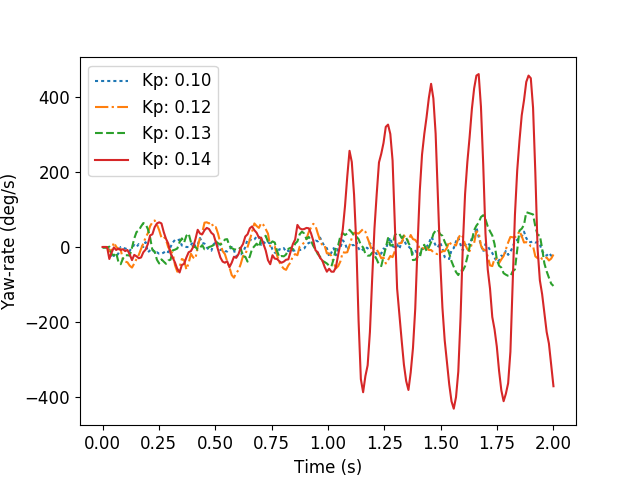
\includegraphics[width=\textwidth]{pics/straight_ku.png}
		\caption{Determining the ultimate gain}
		\label{fig:ultimate_gain}
	\end{subfigure}
	\begin{subfigure}[b]{0.49\textwidth}
		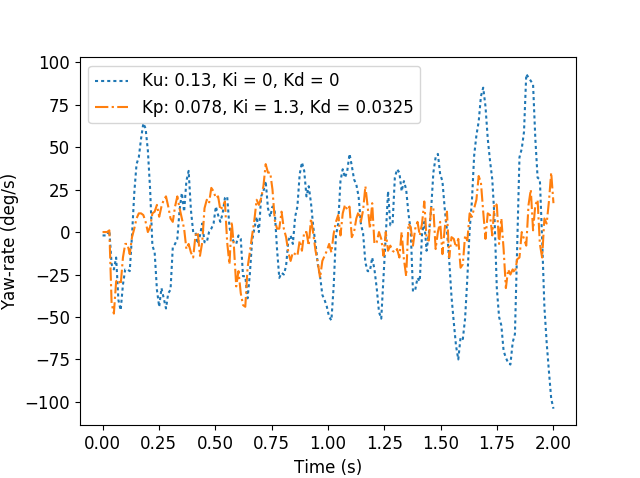
\includegraphics[width=\textwidth]{pics/straight_ku_with_tu.png}
		\caption{Determining the ultimate period}
		\label{fig:gain_tuning}
	\end{subfigure}
	\caption{Tuning the PID controller using the ultimate gain method, first the ultimate gain is determined to be equal to 0.13. Then the ultimate period is determined equal to 0.2 and using Table \ref{tab:gain_chart} the tunable gains are determined.}
\end{figure}

%\subsubsection{Controlled turns}

%The control loop for controlled turning uses the angle, which is obtained by integrating the yaw-rate sensor data from the gyroscope.
%A P controller is used to rotate the robot to the desired angle, the proportional gain is directly influencing turn speed of the robot.
%The motor control values are set to run the motors opposite directions and are equal to the output of the P controller.
%These values will keep decreasing until the robot rotates to the desired angle.


\section{Software Implementation}
\label{sec:dai_software_implementation}

The software implementation that allows the robot to perform controlled movements is divided in three parts, the main program, a control loop and motor control.
In the main program a set of movements can be defined for the robot to be executed.
The robot can be controlled using three movement commands, one for straight trajectories; (1) straight trajectories, (2) curved right turns and (3) curved left turns.
For each movement an additional movement target needs to be defined that specifies the duration, i.e. when the control loop can consider the movement to be finished.

\subsection{Control loop}

When the control loop is instructed to execute a movement, yaw-rate set point, movement target and motor duty cycle target are set accordingly.
A timer running at a frequency of a 100\,Hz, is used to periodically call an interrupt service routine (ISR) and execute the control loop.
Using an ISR has the benefit of a constant sample time, which simplifies the PID loop, because the integration and differentiation time are also constant and known in advance.
If the ISR is triggered, first a yaw-rate sample is requested from the gyroscope.
Based on the current movement, an evaluation is performed to determine if the movement target is reached.
If this is not the case, the yaw-rate is supplied to the PID controller, which in turn updates the motor values.
The output is subtracted from the left motor value and added to the right motor value, in order to keep the average speed approximately the same.

\subsubsection{Movement target}

For straight movements the movement target is equal to a predetermined time, i.e. number of control loop timer trigger events.
Curved movements use an angle movement target.
By integrating the angular velocity an angle estimate is obtained, which is used to verify if the provided angle movement target is reached within a margin of two degrees.
The loop will exit automatically when the required movement target is reached.

\subsection{Motor Control}
% -Write how the pwm control signals are generated for the H-bridge.
The motors are controlled using PWM signals generated by a second timer, which runs at the predetermined frequency of 2\,kHz.
The timer is able to directly control the four IO-ports connected to the H-bridge, eliminating the overhead of an ISR.
The H-bridge is configured such that two IO-ports directly control a motor.
If one of the ports is enabled the motor rotates forwards and if the other port is enabled the motor rotate backwards.
The control loop updates the compare registers corresponding to each of the ports.
The minimum duty cycle value is added to each motor value and is bounded by the maximum duty cycle.
When the timer reaches a value that corresponds to a value one of the compare registers the connected port is toggled automatically.

%\subsection{Controlled Turns}
%The set point is assumed to be reached when the angle is within two degrees of the target, in this case the loop will stop automatically.
%To allow enough precision to measure if the target is within these two degrees, the timer which executes the control loop was set to run at 100\,Hz.
%Secondly, the proportional gain should not be set to low because the robot might not able to reach the target but also not to high as it can overshoot the target.

\subsection{Persistent Movement}
The transiently-powered robot can make one movement or a series of movements, which probably require multiple power cycles to complete.
To be able to finish a movement and not reset, i.e. redo the same movement, a simple checkpointing method is used to save the progress across power cycles.
A persistent counter registers the progress in the set of movements.
Every control loop iteration the persistent variable that captures the progress towards the movement target is updated, and depending on the movement can be a time or angle.
The right and left motor speed tuned by the PID controller are not saved and restored after a power interrupt.
Due to the startup phase of the motors, previously tuned motor speeds are suspected to be invalid and cannot be used after a power interrupt. 

\subsection{Extendability}
The current software implementation consists of 700 lines of MSP430 specific C code, which compiled take up 14\% of the SRAM and 14\% of the FRAM.
The control loop is implemented using an ISR leaving the main processor available for other computation tasks.
The backscatter communication channel on the WISP is currently not implemented, but can potentially be used to provide communication with a global host. 
Two of the five available timers are used for the control loop and the motor control, while the other three timers are used by the WISP software communication stack.